\chapter{Introduction}

Biology and nature have always been imitated in art and science, and over the years the imitations are growing increasingly better. Artificial Intelligence (AI) and its sub-field of Machine Learning (ML) is one of these areas. While ML is a valuable tool in itself, the ultimate goal of AI is to build what is referred to as \textit{Artificial General Intelligence}: A system capable of not only human-level performance in one field but able to generalize across task-domains and teach itself multiple new skills. 

As we again draw upon nature for inspiration and insights into how such a system might be constructed, the brains capability of learning new skills based on old ones is one ability it seems necessary our future artificial minds possess. Who of us can recall something they learned that was without any previous knowledge to base it on? Before children learn to multiply, they learn how to add. The time before that is spent counting fingers. Even riding a bike requires a level of balance and understanding of locomotion developed in infancy.

The walnut-shaped learning machine inside our skulls consists of billions of neurons. These transmit information in the form of energy through a vast network of synaptic connections and causes all forms of brain activity from contemplation to fight-or-flight responses. Drawing upon the structure of this cell, the Artificial Neuron was constructed in an attempt to model and imitate the learning ability of the human mind. Where the stimulation of a neuron causes it to activate and pass on the stimuli through its \textit{axon}, the artificial neuron is fed numbers through its inputs. These are processed arithmetically and output through its artificial synapses. Structuring these artificial neurons in a network, where the output of one neuron is fed as input to other, creates a \textit{Artificial Neural Network}\footnote{Often just called Neural Network or NN in the context of Machine Learning.} (ANN). 

The learning in such an ANN is achieved by every input to an artificial neuron being weighted by a tunable parameter, the amount of which governs the networks \textit{capacity}\footnote{A networks capacity describes the amount of knowledge it can retain and is set by the number of parameters in the network.}. These parameters are optimized in such a way that the output of the entire network has the smallest error possible. This way of representing knowledge in parametric space has proved itself quite useful for problem-solving, but the troubles arise when applying the artificial neural network to multiple problems at the same time.

\section{Motivation}
Our brains are capable of learning something based on previous knowledge without distorting that reused knowledge. A standard Artificial Neural Network, on the other hand, would have to change its parameters to learn a task, which distorts the state they were already in. This distortion, as discussed in section \ref{background:catastrophicforgetting}, is called \textit{catastrophic forgetting}.

Multiple types of solutions are proposed to this problem. \emph{Orthogonalization techniques}\cite{Orthogonal} puts restrictions on the learning algorithm and encourage sparse activation of hidden layers. Similarly, \emph{Elastic Weight Consolidation}\cite{ewc} (EWC) makes sure learning is slowed down in parameters important to old tasks. This is to keep the parameters in areas of high performance for all problems. \emph{Interleaved learning}\cite{interleavedlearning} approach the problem of catastrophic forgetting differently. By training on old examples in-between and during training on new data, old knowledge can be retained. However, this requires storing old input-output pairs if challenges are faced concurrently.

Other solutions resolve the problem by using different network architectures. Ellefsen et. al\cite{kai} used biologically inspired algorithms to evolve small networks that for two types of input, learn to adopt a \textit{modular} structure. This structure was capable of retaining knowledge that was not forgotten as training scenarios changed during experiments. 

Another approach where invulnerability to catastrophic forgetting is achieved by architectural design is the \emph{Progressive Neural Network}\cite{progressiveneuralnetworks} (PNN). By scaling the network with new parameters for each problem, PNN has no restrictions on the type of tasks applied to the network, since each problems parameters can occupy the most suitable parameter-space. By allowing the reuse of parameters previously optimized while not allowing them to change, each new problem might be solved by leaning on old experiences. However, the scaling of such a network can quickly create a large, unwieldy structure only usable with computationally capable machines. To ensure enough parameter resources for each new task, the amount of network capacity needed is usually overestimated, which only compound the problem. 

Building on the PNN work, DeepMind proposed a new solution to catastrophic forgetting in 2017, the \emph{PathNet} structure\cite{pathnet}. Similarly to PNN, PathNet solves catastrophic forgetting by allocating new parameters for each task, while allowing the unaltered reuse of previously trained parameters. Which sets of parameters allocated for each task is determined by a search through all permutations of trained and untrained modules of parameters.

\section{Goal}
Both the strength and weakness of PNN is its scaling. While it does not cap the number of tasks the structure can learn, it can keep growing indefinitely it allowed. The PathNet, on the other hand, is instantiated with a capacity that is kept constant, meaning new tasks does not change the structure. Each new tasks allocates parameters to its cause, causing the available capacity to shrink. Optimizing PathNet's ability to reuse as much of the capacity it needs for a task instead of training it from scratch would directly increase the number of problems it can solve. 

The focus of this thesis will be to introduce new insights into the reuse of knowledge in a modular learning scenario with the PathNet structure\cite{pathnet} without placing limitations on the performance of each solution. Reusing knowledge for the sake of reuse is in itself, is not beneficial to the cause of Machine Learning. Parameters can always be chosen arbitrarily if its effect on accuracy is of no importance. The goal is to limit the wasted training effort spent on relearning "memetic"\footnote{Memetic is used here to describe a quantification of knowledge in the same way "meme" is used by Richard Dawkins\cite{selfishGene} to describe a unit of cultural knowledge, here as a unit of knowledge used to solve a task.} knowledge already retained in the network. 

Addressing this goal, three experiments in chapter \ref{exp1}, \ref{exp2}, and \ref{exp3} raise questions about how the search for optimal parameter-permutations affect the reuse of those parameters and the performance of the permutation. Figure \ref{fig:research_questions} shows what types of questions are raised in each experiment, and how they are related to each other. 

\begin{figure}[t]
    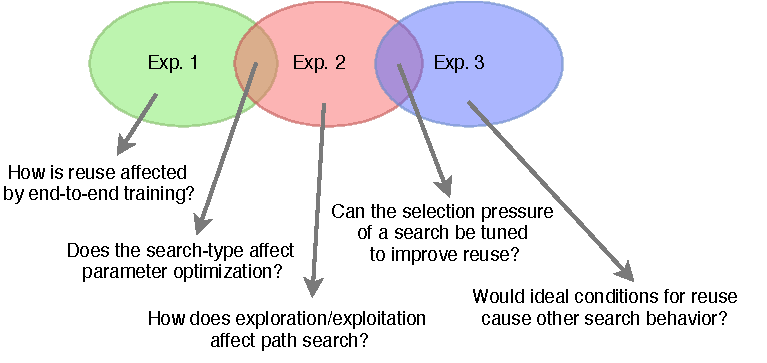
\includegraphics[width=\textwidth]{Chapters/1.Introduction/figures/All_experiments.pdf}
    \caption[Thesis questions]{Visualization of how the questions raised in this thesis is separated across the three experiments.}
    \label{fig:research_questions}
\end{figure}

Chapter \ref{exp1} investigate the possibility of arbitrarily selecting the first set of parameters for end-to-end training, instead of performing a time-consuming search through randomly initialized weights. This might save time in future experiments as there is no knowledge to reuse when the first task is learning. However, the end-to-end training might affect the optimization of the selected weights and increase the difficulty of reusing them in future tasks. A more general statement of this goal is to test if different search types and parameter training contexts affect parameter \textit{reuse}. If the results from this experiment indicate that there is no difference in parameter reuse between the two training schemes for the first task, subsequent experiments will be performed using this arbitrarily selecting of the first parameter set. 

Experiment two in chapter \ref{exp2} share the research goal of testing if different search schemes affect learning, but under a more extensive multi-task scenario with six tasks. The experiment explores how the knowledge reuse is affected by different search types, and if a search scheme can be selected to optimize this reuse. Seven algorithms are tried, where the \textit{selection pressure}(see section \ref{background:GA}) of each algorithm is different. 

The last experiment in chapter \ref{exp3} deploy the same search algorithms used in chapter \ref{exp2} in a scenario optimal for knowledge reuse. By learning the same tasks two times, all the necessary knowledge for solving the second problem is present in the PathNet. As an ideal search algorithm should be able to find the best-suited parameters for each task, this scenario might unveil interesting differences between the algorithms. The seven algorithms are tried with four different termination limits to the search to investigate if the knowledge reuse follows other patterns at different points during the search. 


\section{Thesis Outline}
\subsubsection{Chapter 1. Introduction}
Providing an introduction to the thesis as well as the motivation behind it.
\subsubsection{Chapter 2. Theoretical Background}
Lays the theoretical foundation drawn upon in this thesis. The previous work done on the PathNet structure is mentioned her.
\subsubsection{Chapter 3. Implementation}
Information about code implementation and what data is used.
\subsubsection{Chapter 4. Experiment 1: Selection versus search}
The first experiment where module permutation is done in an empty PathNet structure. The experiment explores the possibility of not performing a full path search for the first path, but rather selecting the first modules arbitrarily.
\subsubsection{Chapter 5. Experiment 2: Selection pressure}
Exploring search algorithms used for optimal module selection. Multiple searches are performed where the selection pressure of the search algorithms are different. 
\subsubsection{Chapter 6. Experiment 3: Relearning a task}
Searching for an optimal path through a PathNet to solve a task which the structure already knows. Testing if the different algorithms have search properties which provide better or worse knowledge reuse.
\subsubsection{Chapter 7. Discussion and conclusion}
Concluding the thesis is a summary of observations and conclusions drawn from the experiments.

\iffalse

\section{Motivation}
Our brains are capable of learning something based on previous knowledge without distorting that reused knowledge. This distortion, as discussed in section \ref{background:catastrophicforgetting}, is called catastrophic forgetting and is a problem addressed and to some degree solved by technologies such as EWC\cite{ewc}, PNNs\cite{progressiveneuralnetworks} and the PathNet structure\cite{pathnet}. These introduce the ability to retain parameters optimized for a previously learned task while a new task is introduced. 

However, these three solutions have limitations. EWC optimize the same set of parameters to multiple tasks, which puts restrictions on which area in parameter-space the model can occupy. PNN and PathNet both are theoretically unlimited in the number of tasks they can retain. In practice, however, restrictions on hardware and feasible training time governs the number of tasks and parameters in these structures. 

Optimizing the reuse of parameters between tasks can reduce the overall need for new capacity for each task. Efficiently applying old knowledge to new problems could, therefore, be a step towards creating vast multi-task learning systems. 

\section{Goal}
To investigate the possibilities of effective knowledge reuse, this thesis explores the PathNet structure. A Super Neural Network which forgoes the monolithic architecture of traditional machine learning models in favor of a modular approach to parameter optimization. The three experiments will address how the modular training affects the transferability of knowledge between tasks and in what area of the exploration/exploitation landscape a search algorithm should be focused.
\fi





\iffalse
\section{Problem/hypothesis}

where do i start?
Question DeepMind left unanswered is how different GAs influence task learning and module reuse. 
Exploration vs exploitation\ref{background:GA}

why this? broad answers first, specify later. 
We know PN works. would it work better for different algorithms?
logical next step from original paper "unit of evolution"




* What do modular PN training do with the knowledge? 
- More/less accuracy?
- More/less transferability? 
Test by learning in end-to-end first then PN search. 
Difference in performance or reuse?

* Can we make reuse easier by shifting focus of search algorithm?
- PN original: Naive search. Higher exploitation improve on module selection?

\section{How to answer?}
- Set up simple multitask scenarios and try. 
* 2 tasks where first are end to end vs PN
* List algorithms with different selection pressure and try on multiple tasks. 


    What is the use of a Nifty Gadget? 
    What is the problem? 
    How can it be solved? 
    What are the previous approaches? 
    What is your approach? 
    Why do it this way? 
    What are your results? 
    Why is this better? 
    Is this a new approach? 
    Why haven't anyone done it before? 
    or
    Why do you reiterate previous work? 
    What is your contribution to the field of Nifty Gadgets? 
    
    \section{What should this chapter contain?}
    Presentation of the problem or phenomenon to be addressed, the situation where the problem or phenomenon occurs, and references to earlier relevant research. 
    \subsection{Common errors}
    Problem is not properly specified or formulated; insufficient references to earlier work.  
    
    \section{Purpose}
    What can be gained by more knowledge about the problem or phenomenon. 
    \subsection{Common errors}
    The purpose is not mentioned, not connected to earlier research, or not in line with what the actual contents of the thesis.  
    
    \section{Problem/Hypothesis} 
    Questions that need to be answered to reach 
    the goal and/or hypothesis formulated be means of 
    underlying theories. 
    \subsection{Common errors}
    Missing problem description; deficiencies in the connections between questions; badly formulated 
    hypothesis.  
    
    \section{Method} 
    Choice of an adequate method with respect to the 
    purpose and problem/hypothesis. 
    
    \subsection{Common errors}
    An inappropriate method is used, for example due to lack of knowledge about different methods; 
    erroneous use of chosen method.  
\fi